\documentclass[twoside,10pt]{article}
\usepackage{amsmath,amsfonts,amsthm,fullpage,amssymb}
%\usepackage{mymath}
\usepackage{algorithm}
\usepackage{algorithmic}
\usepackage{graphicx}
\usepackage{url}
\usepackage{subcaption}


\begin{document}


\title{ISYE 6740 Homework 4\\ 
Summer 2020\\
\small Total 100 points.}
\author{Arjun Singh}
\date{\today}
\maketitle



%As usual, please submit a report with sufficient explanation of your answers to each the questions, together with your code, in a zip folder.

%----------------------------------------------------------------------------------



\begin{enumerate}


\item{\bf SVM. } (30 points)

\begin{enumerate}
\item (10 points) Explain why can we set the margin $c = 1$ to derive the SVM formulation?
\begin{itemize}
\item Answer:\\
When deriving the margin for SVM, the value of $c$ simply scales $w$ and $b$ and hence does not change the relative goodness of different classifiers. Therefore, we can set $c = 1$ to obtain a simpler optimization problem.
\end{itemize}
\item (10 points) Using Lagrangian dual formulation, show that the weight vector can be represented as
\[
w = \sum_{i=1}^n \alpha_i y_i x_i.
\]
where $\alpha_i \geq 0$ are the dual variables. What does this imply in terms of how to relate data to $w$?
\begin{itemize}
\item Answer:\\
The standard form of the problem is:
$$\min\limits_{w,b} \frac{1}{2} w^\intercal w \quad s.t. \quad 1 - y^i(w^\intercal x^i + b) \leq 0, \forall i$$
Converting to the Lagrangian form:
$$ L(w,b,\alpha) = \frac{1}{2} w^\intercal w + \sum_{i=1}^m \alpha(1 - y^i(w^\intercal x^i + b))
$$

To obtain the weight vector, we can take the derivative of $L$ w.r.t $w$ and set it equal to 0.
$$ \frac{dL}{dw} = w - \sum_{i=1}^m \alpha_i y^i x^i $$
$$ 0 = w - \sum_{i=1}^m \alpha_i y^i x^i $$
$$\implies w =  \sum_{i=1}^m \alpha_i y^i x^i$$

This implies that the weights $w$ are a linear combination of the input data and labels as well as $\alpha$. The non-zero $\alpha$ in this case will correspond to the support vectors.

Reference:
http://web.mit.edu/6.034/wwwbob/svm-notes-long-08.pdf

\end{itemize}
\item (10 points) Explain why only the data points on the ``margin'' will contribute to the sum above, i.e., playing a role in defining $w$. Hint: use the Lagrangian multiplier derivation and KKT condition we discussed in class. 
\begin{itemize}
\item Answer:\\
According to the KKT conditions, $\alpha_i g_i (w) = 0$. Any point that is not on the margin will have $g_i(w) < 0$, which implies that $\alpha = 0$. For points that are on the margin, $g_i(w) = 0$, which implies $\alpha_i > 0$. Therefore the points with non-zero $\alpha_i$ represent the support vectors.
\end{itemize}

\end{enumerate}



\item{\bf  Simple SVM by hand.} (20 points)

Suppose we only have four training examples in two dimensions as shown in Fig. The positive samples at $x_1 = (0, 0)$, $x_2 = (2, 2)$ and negative samples at $x_3 = (h, 1)$ and $x_4 = (0, 3)$. 
%
\begin{center}
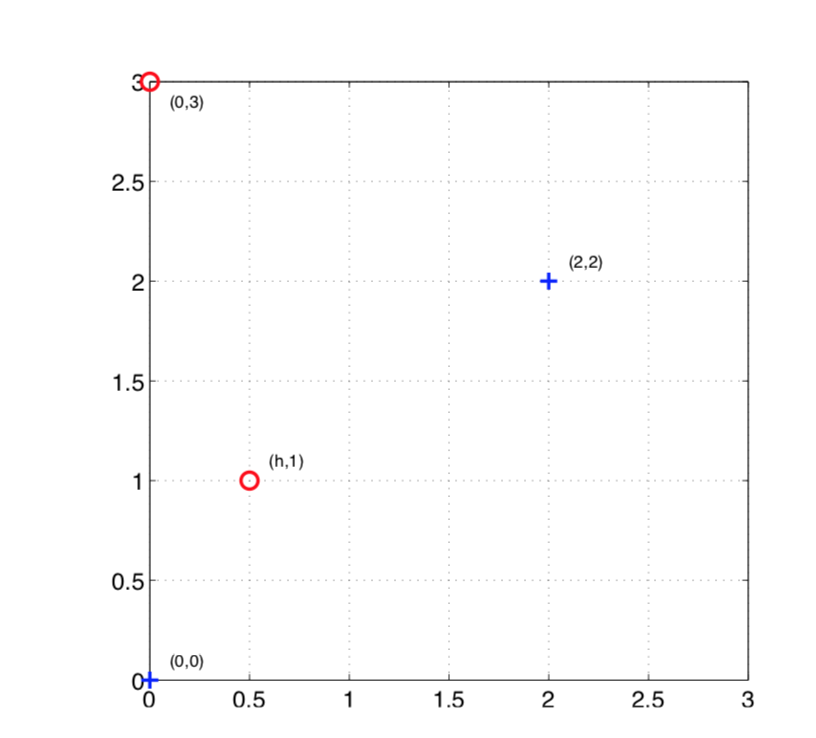
\includegraphics[width = 0.5\textwidth]{svm}
\end{center}

\begin{enumerate}
\item (10 points) For what range of parameter $h > 0$, the training points are still linearly separable?
\begin{itemize}
\item Answer\\
For the training points to be linearly separable, $h<1$ or $h>4$.
\end{itemize}


\item (10 points) Does the orientation of the maximum margin decision boundary change as $h$ changes, when the points are separable?
\begin{itemize}
\item Answer\\
Yes, when $h<1$, the slope of the decision boundary is positive and increasing as $h$ gets smaller. When $h>4$, the slope of the decision boundary is negative and get smaller in magnitude as $h$ increases.
\end{itemize}
\end{enumerate}



\item {\bf Neural networks.} (20 points)

\begin{enumerate}
\item (10 points)
Consider a neural networks for a binary classification using sigmoid function for each unit. If the network has no hidden layer, explain why the model is equivalent to logistic regression. 
\begin{itemize}
\item Answer:\\
A neural network has an input layer, hidden layers and an output layer. Each perceptron takes in a linear combination of the inputs and weights and produces an output based on an activation function. For a binary classification problem, if the neural network has no hidden layer, we end up with the following network:
\begin{center}
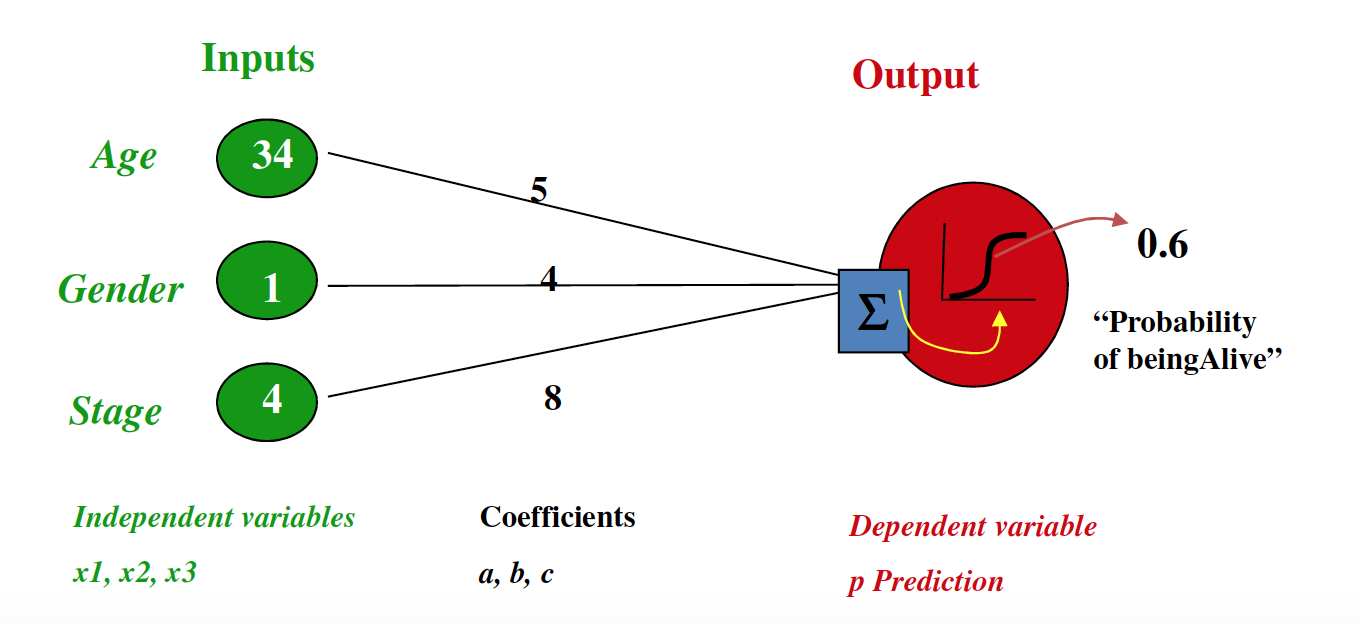
\includegraphics[width = 0.5\textwidth]{NeuralNet.png}
\end{center}

In this example, the input layer leads directly to the output perceptron. The activation function for this perceptron is the logistic function that produces a probability for the output, which is the same as a logistic regression model. Hence, the logistic regression can be thought of as a special case of a neural network when there are no hidden layers.
Image source: Lecture slides
\end{itemize}
\item (10 points) 
Consider a simple two-layer network in the lecture slides. Given $m$ training data $(x^i, y^i)$, $i = 1, \ldots, m$, the cost function used to training the neural networks
\[
\ell(w, \alpha, \beta) = \sum_{i=1}^m (y^i - \sigma(w^T z^i))^2
\]
where $\sigma (x) = 1/(1+e^{-x})$ is the sigmoid function, $z^i$ is a two-dimensional vector such that  $z_1^i = \sigma(\alpha^T x^i)$, and $z_2^i = \sigma(\beta^T x^i)$. Show the that the gradient is given by
\[
\frac{\partial \ell(w, \alpha, \beta) }{\partial w}
= - \sum_{i=1}^m 2(y^i - \sigma(u^i))\sigma(u^i)(1-\sigma(u^i)) z^i,
\]
where $u^i = w^T z^i$. Also find the gradient of $\ell(w, \alpha, \beta)$ with respect to $\alpha$ and $\beta$ and write down their expression.
\begin{itemize}
\item Answer:\\

$$
\ell(w, \alpha, \beta) = \sum_{i=1}^m (y^i - \sigma(w^T z^i))^2
$$

$$ \frac{d \ell}{dw} = \sum_{i=1}^m 2(y^i - \sigma(w^T z^i)) \cdot -\frac{d \sigma(w^T z^i)}{dw}$$

Given that $u^i = w^T z^i$, where $u^i$ is the sigmoid function:

$$ \frac{d \ell}{dw} = \sum_{i=1}^m -2(y^i - \sigma(u^i)) \cdot \frac{d \sigma(u^i)}{dw}$$

The first derivative of the sigmoid function is given by:

$$ \frac{d\sigma(u^i)}{du} = \sigma(u^i)(1-\sigma(u^i))$$

Plugging this back in, we get:

$$ \frac{d \ell}{dw} = \sum_{i=1}^m -2(y^i - \sigma(u^i)) \cdot \sigma(u^i)(1-\sigma(u^i))$$

Replacing $u^i$ with $w^T z^i$, we get an additional $z^i$ term at the end

$$ \frac{d \ell}{dw} = \sum_{i=1}^m -2(y^i - \sigma(w^T z^i)) \cdot \sigma(w^T z^i)(1-\sigma(w^T z^i)) \cdot z^i$$

$$ \implies \frac{d \ell}{dw} = \sum_{i=1}^m -2(y^i - \sigma(u^i)) \cdot \sigma(u^i)(1-\sigma(u^i)) \cdot z^i$$

Similarly, we can find the gradient of $\ell$ w.r.t $\alpha$ and $\beta$. Given that $z_1^i = \sigma(\alpha^T x^i)$ and $z_2^i = \sigma(\beta^T x^i)$:

$$
\ell(w, \alpha, \beta) = \sum_{i=1}^m (y^i - \sigma(w^T z^i))^2
$$

$$ \frac{d \ell}{d \alpha} = \frac{d \ell}{d z_1^i} \frac{d z_1^i}{d \alpha}$$

$$
\frac{d \ell}{d z_1^i} = \sum_{i=1}^m -2 (y^i - \sigma(w^T z_1^i)) \cdot \frac{d \sigma(w^T z_1^i)}{d z_1^i}	
$$

Using results from the previous exercise:
$$
\frac{d \ell}{d z_1^i} = \sum_{i=1}^m -2 (y^i - \sigma(w^T z_1^i)) \cdot 	
\sigma(w^T z_1^i)(1-\sigma(w^T z_1^i) \cdot w^T 
$$

Similarly:
$$
\frac{d z_1^i}{d \alpha} = \frac{d \sigma(\alpha^T x^i)}{d \alpha}
$$

$$
\frac{d z_1^i}{d \alpha} = \sigma(\alpha^T x^i)(1-\sigma(\alpha^T x^i))\cdot x^i 
$$

Combining the equations, we get:

$$ 
\frac{d \ell}{d \alpha} = \sum_{i=1}^m -2 (y^i - \sigma(w^T z_1^i)) \cdot 	
\sigma(w^T z_1^i)(1-\sigma(w^T z_1^i) \cdot w^T \cdot \sigma(\alpha^T x^i)(1-\sigma(\alpha^T x^i))\cdot x^i $$

For simplification, let $u^i = w^T z_1^i$ and $v^i = \alpha^T x^i$
$$ 
\frac{d \ell}{d \alpha} = \sum_{i=1}^m -2 (y^i - \sigma(u^i)) \cdot 	
\sigma(u^i)(1-\sigma(u^i) \cdot w_1 \cdot \sigma(u^i)(1-\sigma(u^i))\cdot x^i $$


By similarity

$$ 
\frac{d \ell}{d \beta} = \sum_{i=1}^m -2 (y^i - \sigma(u^i)) \cdot 	
\sigma(u^i)(1-\sigma(u^i) \cdot w_2 \cdot \sigma(u^i)(1-\sigma(u^i))\cdot x^i $$


\end{itemize}
\end{enumerate}


\item {\bf Comparing SVM and simple neural networks.} (30 points)

This question is to implement and compare {\bf SVM and simple neural networks} for the same datasets we tried for the last homework (so in the end, we have compared 5 classification algorithms on two datasets). We suggest to use \textsf{Scikit-learn}, which is a commonly-used and powerful \textsf{Python} library with various machine learning tools. But you can also use other similar libraries in other programming languages of your choice to perform the tasks. 

You may use a neural networks function \textsf{sklearn.neural\_network} with \textsf{hidden\_layer\_sizes=(5, 2)}. Tune the step size so you have reasonable results. You may use \textsf{svc} and tune the penalty term $C$ to get reasonable results. 

\textbf{Part One (Divorce classification/prediction).} (20 points) 

We will compare using the same dataset as the last homework, which is about participants who completed the personal information form and a divorce predictors scale. 

The data is a modified version of the publicly available at \url{https://archive.ics.uci.edu/ml/datasets/Divorce+Predictors+data+set} (by injecting noise so you will not replicate the results on uci website). There are 170 participants and 54 attributes (or predictor variables) that are all real-valued. The dataset was the same as the last homework. The last column of the CSV file is label $y$ (1 means ``divorce'', 0 means ``no divorce''). Each column is for one feature (predictor variable), and each row is a sample (participant). A detailed explanation for each feature (predictor variable) can be found at the website link above. Our goal is to build a classifier using training data, such that given a test sample, we can classify (or essentially predict) whether its label is 0 (``no divorce'') or 1 (``divorce''). 

Build two classifiers using SVM and a simple neural networks. First random shuffle the data set. Then use the first $80\%$ data for training and the remaining $20\%$ for testing. If you use \textsf{scikit-learn} you can use \textsf{train\_test\_split} to split the dataset. 

\begin{enumerate}

	\item (10 points) Report testing accuracy for each of the two classifiers.  Comment on their performance: which performs better and make a guess why it performs better in this setting. 
	
	\begin{itemize}
	\item Answer:\\
	After training the clasifiers with 80\% of the data and testing on the remaining 20\%, I achieved the following results
	\begin{center}
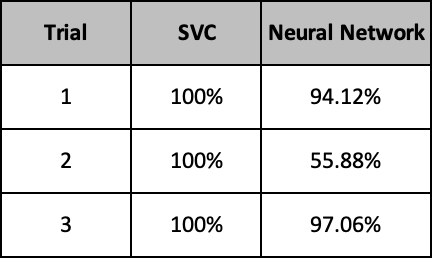
\includegraphics[width = 0.25\textwidth]{Q4a.png}
\end{center}
The SVC classifier has superior performance in all trials. An implication of such good results for the classifier is that the data is linearly separable, which makes it a good problem for a SVM classifier.


	\end{itemize}
	\item (10 points) Use the first two features to train two new classifiers. Plot the data points and decision boundary of each classifier. Comment on the difference between the decision boundary for the two classifiers. Please clearly represent the data points with different labels using different colors.
	
\begin{itemize}
\item Answer:\\
By using only the first 2 features, I achieved the following results:
\begin{center}
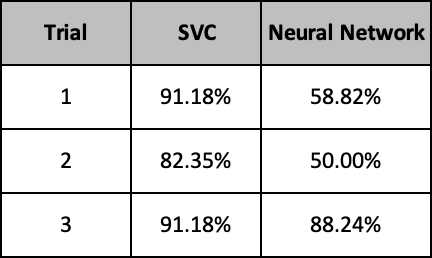
\includegraphics[width = 0.25\textwidth]{Q4b.png}
\end{center}


\begin{figure}
\begin{subfigure}{.5\textwidth}
  \centering
  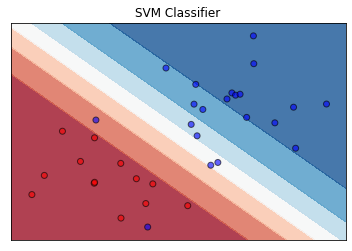
\includegraphics[width=.8\linewidth]{svmboundary.png}
  \caption{SVM}
  \label{fig:sfig1}
\end{subfigure}%
\begin{subfigure}{.5\textwidth}
  \centering
  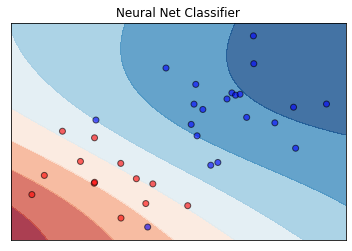
\includegraphics[width=.8\linewidth]{nnboundary.png}
  \caption{Neural Network}
  \label{fig:sfig2}
\end{subfigure}

\caption{Decision Boundaries}
\label{fig:fig}
\end{figure}

Figure 1 displays the decision boundaries for the 2 classifiers. The SVM classifier uses a linear decision boundary whereas the neural network is able to work with non-linear boundaries. Although the neural network does not provided superior performance in this particular scenario, it can be useful for other datasets where the data has non-linear patterns.
\end{itemize}	
	
\end{enumerate}

\textbf{Part Two (Handwritten digits classification).} (10 points) Repeat the above part (a) using the \textbf{MNIST Data} in our \textbf{Homework 3}. Here, give ``digit'' 6 label $y = 1$, and give ``digit'' 2 label $y = 0$. All the pixels in each image will be the feature (predictor variables) for that sample (i.e., image). Our goal is to build classifiers such that given a new testing sample, we can tell it is a 2 or a 6. Using the first $80\%$ of the samples for training and remaining $20\%$ for testing. Report the classification accuracy on testing data, for each of the two classifiers. Comment on their performance: which performs better and make a guess why they perform better in this setting. 

\begin{itemize}
\item Answer:\\
Similar to the exercise above, I achieved the following results on the MNIST dataset:
\begin{center}
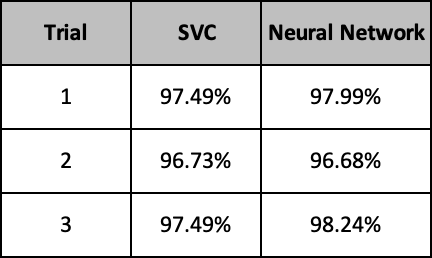
\includegraphics[width = 0.25\textwidth]{MNIST.png}
\end{center}
With the MNIST dataset, it appears that the neural network has slightly better performance. This can be attributed to the fact that the images in the MNIST dataset have non-linear patterns and are unstructured, which make it an ideal problem for neural networks.

\end{itemize}

\end{enumerate}


\end{document}
